\section{Experiments}
\label{sec:experiments}

\subsection{Setup}
\paragraph{Data}
One person recorded 8 egocentric videos of household chores (wiping a counter, folding cloth on a bed, making a bed, wrapping a charger cable at a desk) with a handheld camera, about 10 minutes each. TransNetV2~\cite{transnetv2}, as packaged in Cosmos Curate, split them at shot boundaries into 116 clips, each trimmed to at most 15~s and downsampled to 4~fps and $854\times480$, the input format the Cosmos models expect. The retained set totals about 30 minutes. No robot data is involved; the clips are human demonstrations.

\paragraph{Models and hardware}
Reasoning: the Cosmos 3 Nano reasoning tower~\cite{cosmos3,cosmos3nano}. Prompt writing and filtering: GPT-4o mini~\cite{gpt4omini}. Segmentation: SAM2~\cite{sam2}. Rendering: Cosmos Transfer~2.5~\cite{cosmos25,cosmostransfer25} and Cosmos Predict2 2B Video2World~\cite{cosmospredict2}. All runs were on a single A100 80~GB through Google Colab Pro+. Table~\ref{tab:cost} gives wall-clock per clip.

\begin{table}[t]
\centering
\caption{Per-clip cost on one A100 80~GB (Colab Pro+). Reasoning covers detection, ontology and variation proposals. Transfer time is 35 denoising steps at 31~s each plus about 2~min of control-map preprocessing; Predict2 is 35 steps at 6~s each. The dollar figure is the GPT-4o mini API cost over all 116 clips.}
\label{tab:cost}
\small
\begin{tabular}{@{}llS[table-format=2.1]l@{}}
\toprule
Stage & Breakdown & {Time / clip} & Unit \\
\midrule
Cosmos 3 Nano reasoning & boxes + ontology + proposals & 2.2 & min \\
GPT-4o mini filter + prompt & all 116 clips & {$\approx$\,\$0.12} & total \\
Cosmos Transfer 2.5 render & 35 steps $\times$ 31~s + 2~min maps & 20 & min \\
Cosmos Predict2 2B render & 35 steps $\times$ 6~s & 3.5 & min \\
\bottomrule
\end{tabular}
\end{table}

\paragraph{What was generated}
We ran the reasoning stage on all 116 clips and rendered 64 appearance variants of 10 source clips with Cosmos Transfer, about six variations per clip. The figures in this section show renders of four of those clips (counter wiping, cloth folding, bed making, cable wrapping) under the prompts listed in Appendix~\ref{app:prompts}, chosen because they span the single-surface, multi-texture and shape-collapse behaviors we observed across the set. Two Predict2 renders were made for action-level variation. Evaluation is by inspection of matched frames and by the masked color-difference measurement of Sec.~\ref{sec:leakage}. No policy was trained on the output; Sec.~\ref{sec:limits} returns to this.

\subsection{Appearance variation}
\label{sec:appearance}
Fig.~\ref{fig:bucket} shows the counter-wiping clip and its rendered variant for the prompt ``solid blue matte countertop'' with the bucket, towels, hands and lighting named as preserved. The countertop is blue, the hand pose and the bucket geometry are preserved frame for frame, and the motion is the source motion. The variant also differs from the source in ways the prompt forbade: the towels have become blue cloth, the bucket is grey-blue, the wall has warmed from white to beige, the hand is lighter, and a ceiling fixture appears that was never in the source.

\begin{figure}[t]
\centering
\begin{subfigure}{0.49\linewidth}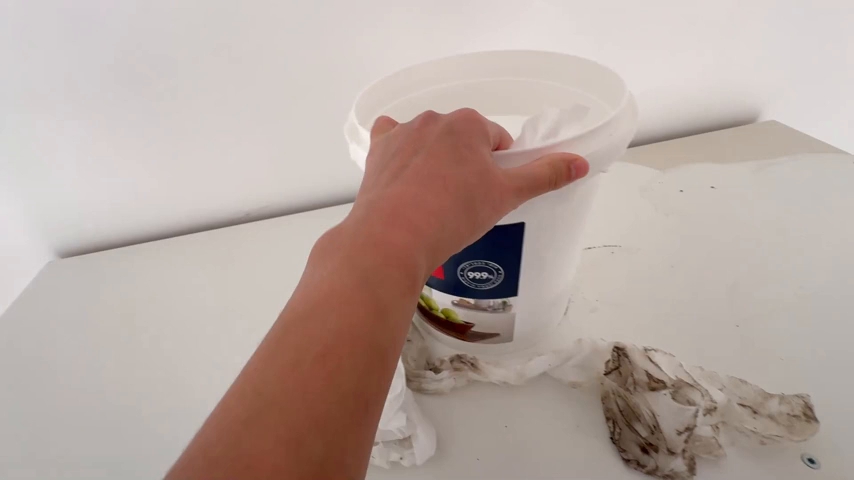
\includegraphics[width=\linewidth]{bucket_orig.png}\caption{source}\end{subfigure}\hfill
\begin{subfigure}{0.49\linewidth}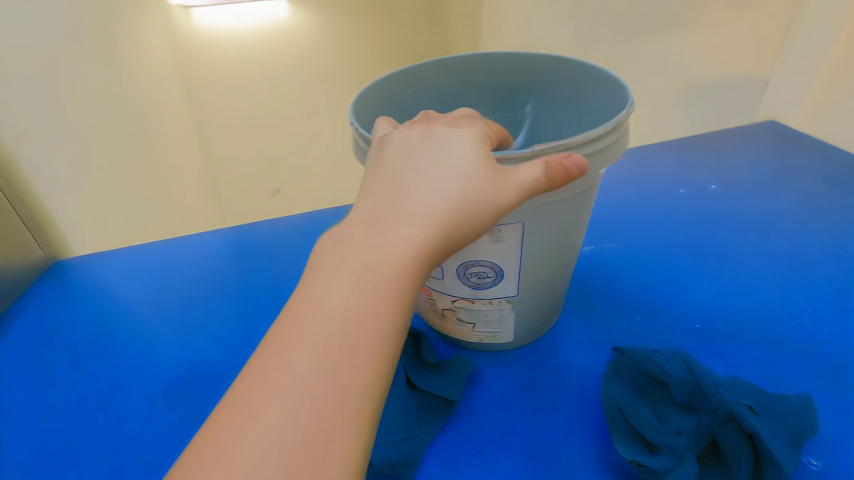
\includegraphics[width=\linewidth]{bucket_gen.png}\caption{variant}\end{subfigure}
\caption{Counter-wiping clip, matched frames. The countertop recolor is the intended edit. The towel, bucket, wall and lighting changes are not; the prompt named each of them as preserved.}
\label{fig:bucket}
\end{figure}

Fig.~\ref{fig:pillow} shows the cloth-folding clip. The prompt asked for a cobalt blue blanket on the left of the bed and listed the white cloth, the patterned pillow, the headboard and a brass ornament as preserved. The render turned nearly every surface blue; the pillow patterns survive only as blue-on-blue relief. Hands are preserved. Fig.~\ref{fig:others} shows the remaining Transfer renders. The desk-and-shelf recolor spread blue onto shelf objects and the cable. The rug prompt for the bed-making clip returned a frame with the correct beige bedspread but heavy smearing and a warped hand, the shape-collapse failure in Table~\ref{tab:weights}. In every case the geometry and the hand motion of the source are retained, and in every case color is applied beyond the target.

\begin{figure}[t]
\centering
\begin{subfigure}{0.49\linewidth}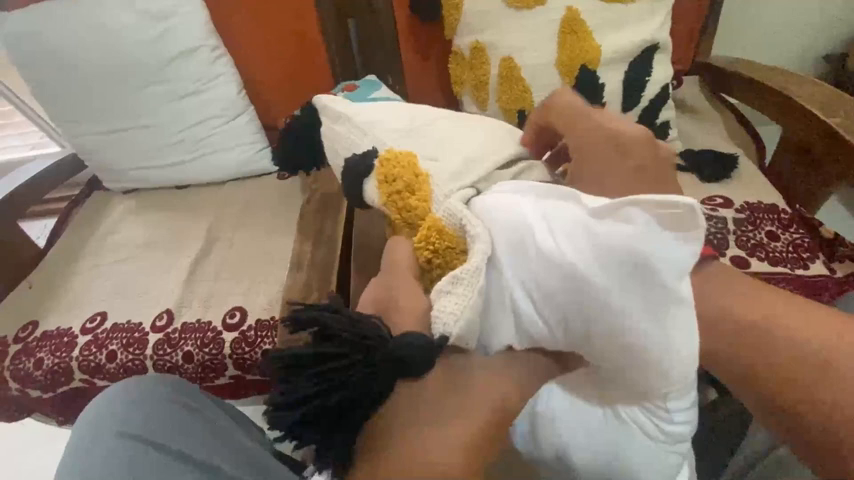
\includegraphics[width=\linewidth]{pillow_orig.png}\caption{source}\end{subfigure}\hfill
\begin{subfigure}{0.49\linewidth}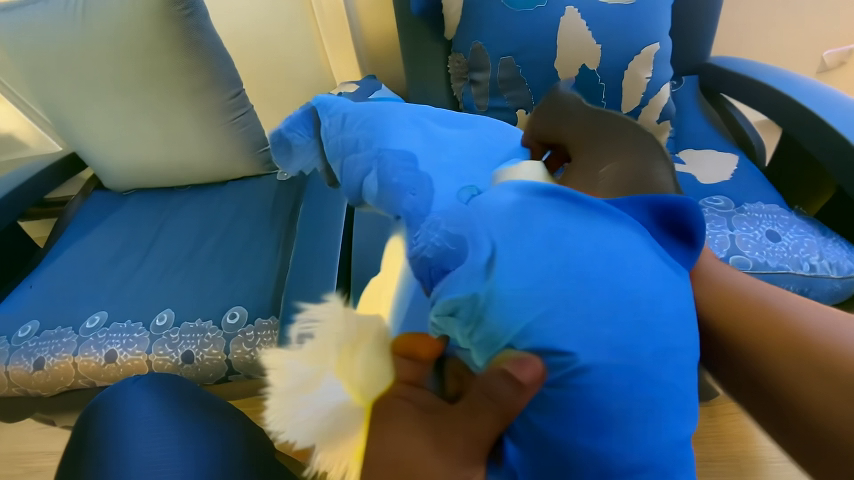
\includegraphics[width=\linewidth]{pillow_gen.png}\caption{variant}\end{subfigure}
\caption{Cloth-folding clip. The prompt targeted a single blanket. The render recolored the cushions, chair and cloth as well. Multi-texture scenes fail more completely than the single-surface case of Fig.~\ref{fig:bucket}.}
\label{fig:pillow}
\end{figure}

\begin{figure}[t]
\centering
\begin{subfigure}{0.23\linewidth}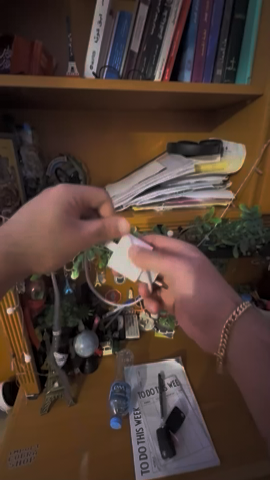
\includegraphics[width=\linewidth]{shelf_orig.png}\caption{desk, source}\end{subfigure}\hfill
\begin{subfigure}{0.23\linewidth}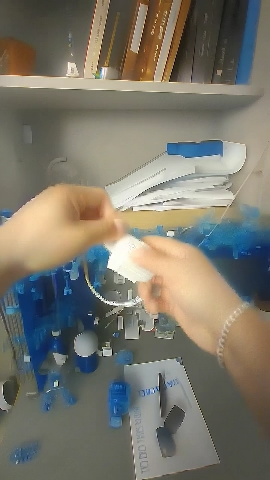
\includegraphics[width=\linewidth]{shelf_gen.png}\caption{blue desk}\end{subfigure}\hfill
\begin{subfigure}{0.48\linewidth}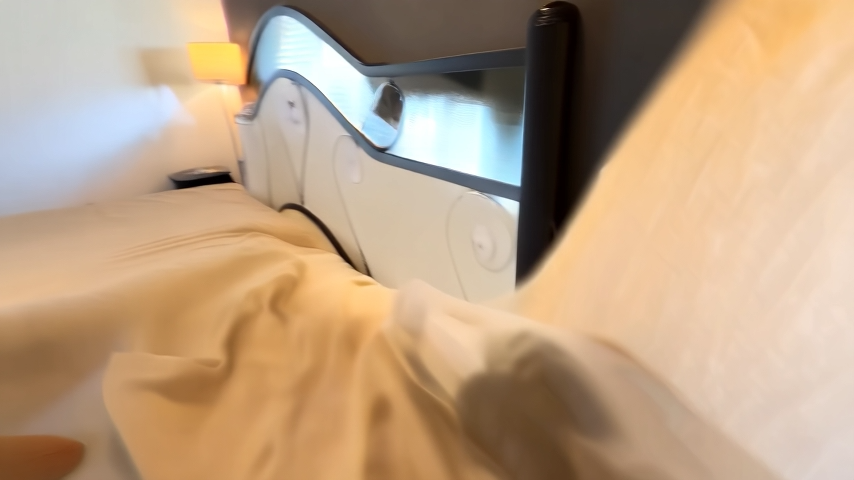
\includegraphics[width=\linewidth]{bed_gen.png}\caption{bed making, navy rug prompt}\end{subfigure}
\caption{Further Transfer renders. (b) Blue leaks from the desk and shelf onto the objects on them. (c) Shape collapse: the bedspread color is right, but surfaces smear and the hand warps.}
\label{fig:others}
\end{figure}

\subsection{Measuring leakage}
\label{sec:leakage}
To put a number on the unintended change, we compare source and variant frame by frame in CIELAB and split the per-pixel CIE76 distance $\Delta E$ by the tracked mask $M$. Pixels inside $M$ are the ones the prompt targeted; pixels outside are the ones it said to preserve. We report the mean over pixels and frames and the fraction of protected pixels whose $\Delta E$ exceeds 10, a difference that is unmistakable to a viewer. Table~\ref{tab:leakage} and Fig.~\ref{fig:leakage} give the result for the counter-wiping clip, the one render for which a usable tracked mask was retained; Sec.~\ref{sec:limits} says what was found for the others.

\begin{table}[t]
\centering
\caption{Masked color difference for the counter-wiping variant, 60 frames. The protected region changes by almost half as much as the target, and nearly all of it changes visibly. Chroma-only distance (a, b channels) shows the change is color, not exposure.}
\label{tab:leakage}
\small
\begin{tabular}{@{}lS[table-format=2.1]S[table-format=2.1]@{}}
\toprule
 & {Target ($M$)} & {Protected ($\bar M$)} \\
\midrule
Mask coverage (fraction of frame) & 0.50 & 0.50 \\
Mean $\Delta E$ & 75.5 & 34.8 \\
Std of per-frame mean $\Delta E$ & 4.0 & 7.2 \\
Mean chroma-only $\Delta E$ & 68.2 & 24.2 \\
Pixels with $\Delta E > 10$ (\%) & {--} & 94.5 \\
Pixels with $\Delta E > 20$ (\%) & {--} & 65.3 \\
\bottomrule
\end{tabular}
\end{table}

\begin{figure}[t]
\centering
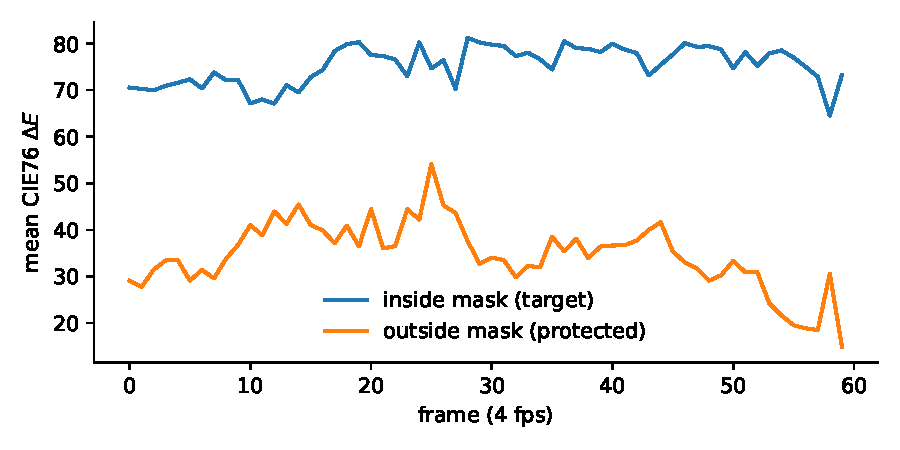
\includegraphics[width=\linewidth]{leakage_per_frame.pdf}
\caption{Per-frame mean $\Delta E$ inside and outside the mask for the counter-wiping variant. The gap is stable across the clip; the protected region never approaches zero.}
\label{fig:leakage}
\end{figure}

\begin{figure}[t]
\centering
\begin{subfigure}{0.32\linewidth}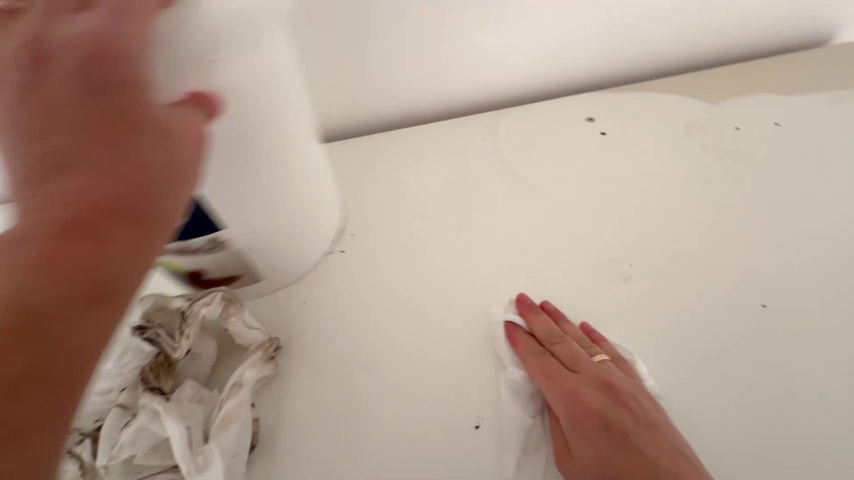
\includegraphics[width=\linewidth]{bucket_orig_f30.png}\caption{source, $t{=}30$}\end{subfigure}\hfill
\begin{subfigure}{0.32\linewidth}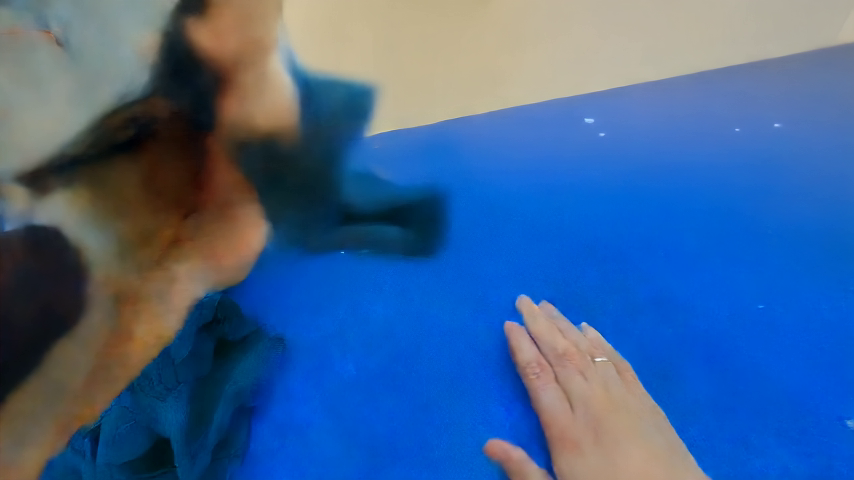
\includegraphics[width=\linewidth]{bucket_gen_f30.png}\caption{variant}\end{subfigure}\hfill
\begin{subfigure}{0.32\linewidth}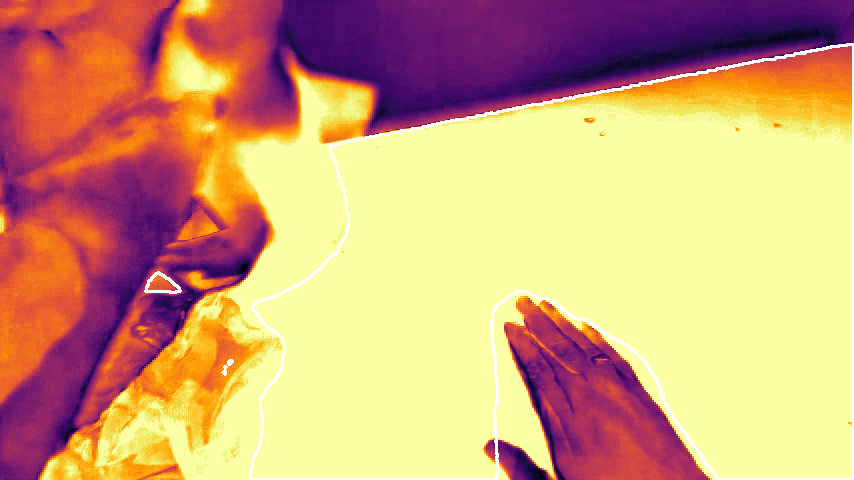
\includegraphics[width=\linewidth]{leakage_heatmap_f30.png}\caption{$\Delta E$}\end{subfigure}
\caption{Spatial distribution of change at frame 30. The white contour is the mask boundary. The towels and bucket (left, outside the mask) change nearly as much as the countertop; the wall (top) changes less but not negligibly.}
\label{fig:heatmap}
\end{figure}

The target region moved by a mean $\Delta E$ of 75, so the recolor itself worked. The protected region moved by 35, and 95\% of its pixels moved by more than 10. The chroma-only columns rule out a mere exposure shift. Fig.~\ref{fig:heatmap} shows where: the towels and bucket, directly adjacent to the target, change almost as much as the target does, and the wall changes less but visibly. With the segmentation control at weight 0.175 and the prompt's preservation clause, the pipeline had two soft mechanisms for containment and neither was sufficient.

\subsection{Control-weight sensitivity}
Table~\ref{tab:weights} summarizes the sweep on the counter-wiping clip. We did not grid-search; each weight was moved until a failure appeared and backed off. Three observations carry over to other clips. Edge weight is the dominant term and is bounded on both sides within a narrow band. Vis must be near zero for any recolor, because the vis branch conditions on the source colors and directly opposes the prompt. Guidance scale trades prompt adherence against realism. At 2 and 3 the model often ignored the variation or applied it weakly; above 5 it followed the prompt and lost the scene, producing frames that no longer read as the same room. All reported renders use 4. We did not find a setting that recolored the target fully and left the protected region unchanged.

\subsection{Action-level variation}
\label{sec:actionresults}
Two action variations from the ontology were attempted with Cosmos Predict2 (35 steps, $848\times480$, 93 frames at 16~fps, seed derived from a hash of the prompt identifier): winding a charger cable around its block one loop at a time with the block held fixed, and a sheet of paper on the desk rotating 90 degrees while three objects on it stay in place (Appendix~\ref{app:prompts}). Both prompts are deliberately specific about what moves, what stays fixed, and how the moving part stays physically attached; the cable prompt even points the model at the input frames as the reference motion. In both renders the forecast frames reproduce the conditioning scene with no visible motion of the cable or the paper (Fig.~\ref{fig:predict}). The model held the scene stable, which is a form of success for a world model, and did not perform the action, which is the only thing we asked of it. We did not fine-tune Predict2; Sec.~\ref{sec:limits} discusses why that is the natural next step.

\begin{figure}[t]
\centering
\begin{subfigure}{0.45\linewidth}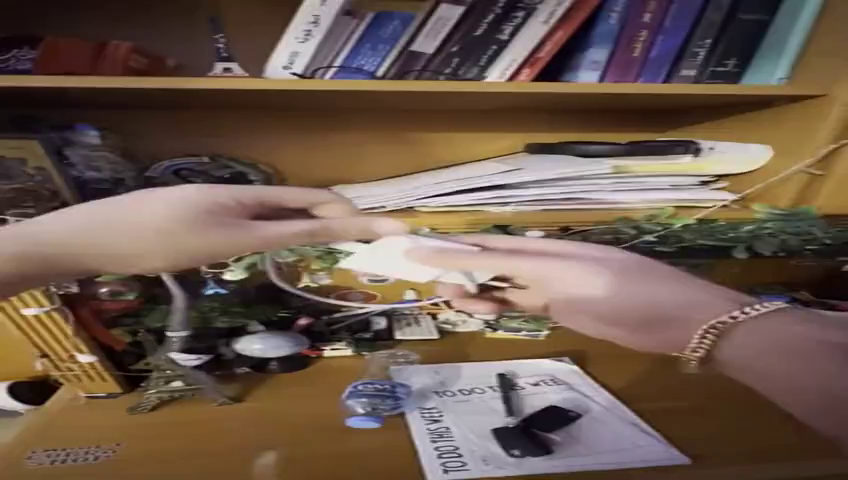
\includegraphics[width=\linewidth]{cord_first.png}\caption{first forecast frame}\end{subfigure}\hfill
\begin{subfigure}{0.45\linewidth}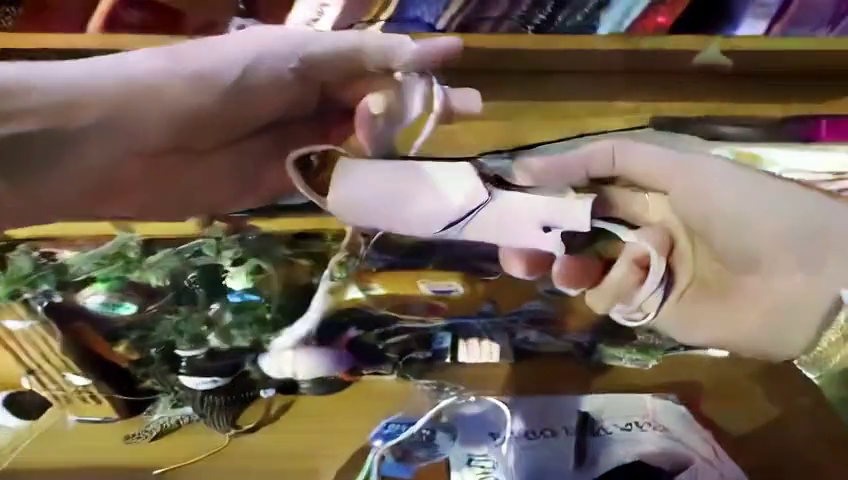
\includegraphics[width=\linewidth]{cord_last.png}\caption{last forecast frame (93)}\end{subfigure}
\caption{Cosmos Predict2 output for the cable-wrapping prompt. The scene is reproduced across the forecast; the cable and hands have not moved.}
\label{fig:predict}
\end{figure}

\subsection{Cost of scaling}
Given the per-clip figures in Table~\ref{tab:cost} and 72 admissible variations per clip from Sec.~\ref{sec:reason}, rendering every variation for every clip would produce $116\times72 = 8{,}352$ variants at about 2{,}800 A100-hours. The 64 we rendered took about 21 GPU-hours. The reasoning and filtering stages are negligible by comparison (a few hours and under a dollar). The render is the entire cost, and it is the stage whose output is not yet contained.
